\section{Characteristics of Large-scale Urban DTNs}
\label{Section3_characteristics}

In this section, we introduce the data set of taxies in Beijing, and analysis the Inter contact time property of the data set.

\subsection{Trace Dataset: Beijing Taxi Traces}
\label{Trace Data}

To study urban DTNs, we use a real-world GPS data which were generated by $12,096$ taxis in Beijing, China within one week (from June 13th to 19th, 2010). This dataset has been used by several key research and application programs of Intelligent Transportation Systems (ITS) in Beijing, China. The number of participated taxis ($12,096$ taxis) is $18\%$ of the total taxis in the city. Each taxi is equipped with a GPS device and upload its information (including location, speed, direction, et al. ) about every 60 seconds. There are about $1.22 \times 10^8$ records in total.
For each row, the record includes a base station ID, company name, taxi ID ($id$), time stamp ($t$), current location ($l$, including both longitude and latitude), another location (out of $54$ fixed locations), speed, acceleration, status of the taxi, event, and height. We only utilize the taxi ID, time stamp, and current location, i.e., $(id,t,l)$, to generate the contacts among taxis for the study.

\subsection{Contact Characteristics in Beijing Taxi Traces}
\label{Contact Characteristics}

%%%%%%%%%%%%%%%%%%%%%%%%%%%%%%%%%%%%%%%%%%%%%%%%%%%5
%%% ׫д��� %%
%%% �󲿷�ICT��ģ���� ָ���ֲ� %%
%%% ���ǵ���һ����������� nodal pair ��˵Ҳ�ʺ� %%
%%% �����ô��ģ������֤ %%
%%%%%%%%%%%%%%%%%%%%%%%%%%%%%%%%%%%%%%%%%%%%%%%%%%%

In the real-world mobility traces of vehicular networks \cite{zaZhuLi-28}, the ICT between two vehicles follows an exponential distribution\cite{qGroeneveltNain-18,vHuWang-23,yJiangLi-26}.Similar conclusions have been found in another Shanghai taxi trace dataset studied by  \cite{zaZhuLi-28,zb20080311017302}. The contact probability between any two nodes based on the global ICT distribution is
 \begin{equation}
    P(X>x)=e^{-\lambda t},
 \end{equation}
where the exponential parameter $\lambda$ reflects the contact strength between nodes. A statistical $\lambda$ can be estimated for the whole network by fitting the global ICT distribution to the exponential function. This simple method can measure the contact strength intuitively and efficiently, and has been frequently used in many DTN routing methods.

In Paper \cite{vHuWang-23}, authors studied the ICT distributions of individual nodal pairs and found that the ICT of a node pair $i$ and $j$ also follows the exponential distribution with exponential parameters $\lambda_{ij}$, according to:
 \begin{equation}\label{equation_label_lambda}
        \lambda_{ij} = n_{ij}/\sum ICT_{ij},
 \end{equation}
where $n_{ij}$ refers to the number of contacts between nodes $i$ and $j$, and $\sum ICT_{ij}$ indicates the total ICTs between these two nodes. Hence, the contact probability of nodes $i$ and $j$ within time period $t$ is
\begin{equation}\label{equation_label_probability}
    p_{ij}(t)=P_{ij}(X\leq t)= 1-e^{-{n_{ij}\over {\sum ICT_{ij}}}t}.
 \end{equation}

\begin{figure}[!h]
\centering
  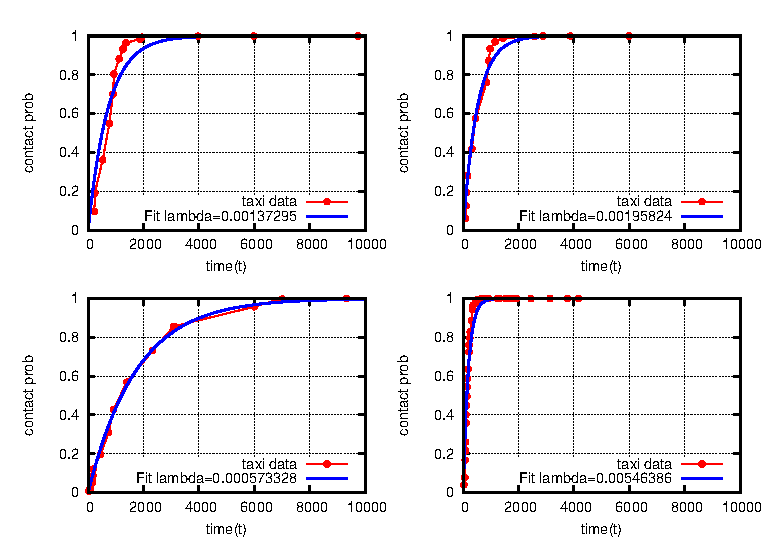
\includegraphics[width=3.5in]{figures_1/multiplot-nodepair.eps}
  \caption{Pairwise ICT distributions of four nodal pairs in Beijing taxi dataset. Red dots are the real sample data from the dataset while blue curves are the fitted exponential distributions.}\label{figure_label_ICT_Distribution}
\end{figure}

By fitting the samples of ICTs for a particular nodal pair with Equation \ref{equation_label_lambda}, we can derive the exponential parameters $\lambda_{ij}$. The values of $\lambda_{ij}$ in Beijing taxi dataset varies significantly from $0.0005$ to $0.005$. Figure \ref{figure_label_ICT_Distribution} shows the exponential distributions fitting for four pairs of nodes.

To further confirm that the method based on pair-wise ICT distributions can characterize the real contact pattern better than the aggregated global ICT distribution, we use the coefficient of determination $R^{2}$ \cite{ozer1985correlation} to determine the similarity degree of modelled ICT curves and real observed curves from dataset. Note that $R^{2}$ is a number between $0$ and $1.0$, and used to describe how well a regression line fits a set of data. An $R^{2}$ near $1.0$ indicates that a regression line fits the data perfectly, while an $R^{2}$ closer to $0$ indicates that a regression line does not fit the data very well.

\begin{figure}[!h]
\centering
  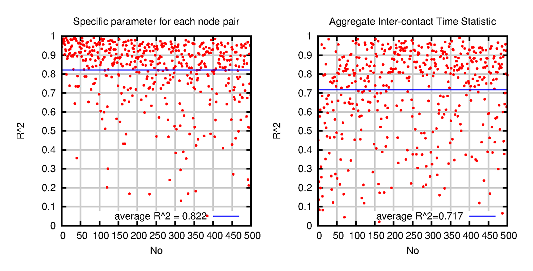
\includegraphics[width=3.5in]{figures_1/R2_comprision.eps}\\
  (a) the pair-wise ICT method \ \ \ \ \ \ \ \ \ \ \ \ \ (b) the global ICT method
  \caption{Comparison of similarities $R^2$ of the two estimation methods. Here, red dots are the values of $R^2$ for $500$ node pairs, while the blue line shows the average value of these $R^2$.}\label{figure_label_Comparison_between_R2}
\end{figure}

For the global ICT method,  we attract the $\lambda$ based on all contact records, and result $\lambda= 0.00077527$. For the pair-wise ICT method, we use Equation  \ref{equation_label_lambda} to learn the individual $\lambda_{ij}$ for each nodal pair. Then we calculate  $R^{2}$  between the estimated distributions based on $\lambda$ or $\lambda_{ij}$ with the real distributions from traces of individual nodal pairs in the dataset. Figure \ref{figure_label_Comparison_between_R2} shows plots of such comparison over  $500$ randomly generated nodal pairs. Clearly, $R^{2}$ differs for each pair of nodes. The blue line in both plots are the average $R^{2}$. The global ICT method has an average of $R^{2}$ at $0.717$ while the pair-wise one is $0.822$. This confirm that using pair-wise ICT distribution can fit the real records better and thus give better contact probability over the global fitting method. Therefore, the contact probability between nodes can by computed by the local information, including the contact time and sum of ICTs, which is beneficial to our distribute clustering and routing process.
